\documentclass[twoside]{book}

% Packages required by doxygen
\usepackage{fixltx2e}
\usepackage{calc}
\usepackage{doxygen}
\usepackage[export]{adjustbox} % also loads graphicx
\usepackage{graphicx}
\usepackage[utf8]{inputenc}
\usepackage{makeidx}
\usepackage{multicol}
\usepackage{multirow}
\PassOptionsToPackage{warn}{textcomp}
\usepackage{textcomp}
\usepackage[nointegrals]{wasysym}
\usepackage[table]{xcolor}

% Font selection
\usepackage[T1]{fontenc}
\usepackage[scaled=.90]{helvet}
\usepackage{courier}
\usepackage{amssymb}
\usepackage{sectsty}
\renewcommand{\familydefault}{\sfdefault}
\allsectionsfont{%
  \fontseries{bc}\selectfont%
  \color{darkgray}%
}
\renewcommand{\DoxyLabelFont}{%
  \fontseries{bc}\selectfont%
  \color{darkgray}%
}
\newcommand{\+}{\discretionary{\mbox{\scriptsize$\hookleftarrow$}}{}{}}

% Page & text layout
\usepackage{geometry}
\geometry{%
  a4paper,%
  top=2.5cm,%
  bottom=2.5cm,%
  left=2.5cm,%
  right=2.5cm%
}
\tolerance=750
\hfuzz=15pt
\hbadness=750
\setlength{\emergencystretch}{15pt}
\setlength{\parindent}{0cm}
\setlength{\parskip}{3ex plus 2ex minus 2ex}
\makeatletter
\renewcommand{\paragraph}{%
  \@startsection{paragraph}{4}{0ex}{-1.0ex}{1.0ex}{%
    \normalfont\normalsize\bfseries\SS@parafont%
  }%
}
\renewcommand{\subparagraph}{%
  \@startsection{subparagraph}{5}{0ex}{-1.0ex}{1.0ex}{%
    \normalfont\normalsize\bfseries\SS@subparafont%
  }%
}
\makeatother

% Headers & footers
\usepackage{fancyhdr}
\pagestyle{fancyplain}
\fancyhead[LE]{\fancyplain{}{\bfseries\thepage}}
\fancyhead[CE]{\fancyplain{}{}}
\fancyhead[RE]{\fancyplain{}{\bfseries\leftmark}}
\fancyhead[LO]{\fancyplain{}{\bfseries\rightmark}}
\fancyhead[CO]{\fancyplain{}{}}
\fancyhead[RO]{\fancyplain{}{\bfseries\thepage}}
\fancyfoot[LE]{\fancyplain{}{}}
\fancyfoot[CE]{\fancyplain{}{}}
\fancyfoot[RE]{\fancyplain{}{\bfseries\scriptsize Generated by Doxygen }}
\fancyfoot[LO]{\fancyplain{}{\bfseries\scriptsize Generated by Doxygen }}
\fancyfoot[CO]{\fancyplain{}{}}
\fancyfoot[RO]{\fancyplain{}{}}
\renewcommand{\footrulewidth}{0.4pt}
\renewcommand{\chaptermark}[1]{%
  \markboth{#1}{}%
}
\renewcommand{\sectionmark}[1]{%
  \markright{\thesection\ #1}%
}

% Indices & bibliography
\usepackage{natbib}
\usepackage[titles]{tocloft}
\setcounter{tocdepth}{3}
\setcounter{secnumdepth}{5}
\makeindex

% Hyperlinks (required, but should be loaded last)
\usepackage{ifpdf}
\ifpdf
  \usepackage[pdftex,pagebackref=true]{hyperref}
\else
  \usepackage[ps2pdf,pagebackref=true]{hyperref}
\fi
\hypersetup{%
  colorlinks=true,%
  linkcolor=blue,%
  citecolor=blue,%
  unicode%
}

% Custom commands
\newcommand{\clearemptydoublepage}{%
  \newpage{\pagestyle{empty}\cleardoublepage}%
}

\usepackage{caption}
\captionsetup{labelsep=space,justification=centering,font={bf},singlelinecheck=off,skip=4pt,position=top}

%===== C O N T E N T S =====

\begin{document}

% Titlepage & ToC
\hypersetup{pageanchor=false,
             bookmarksnumbered=true,
             pdfencoding=unicode
            }
\pagenumbering{alph}
\begin{titlepage}
\vspace*{7cm}
\begin{center}%
{\Large as2-\/project-\/\+Frac7 }\\
\vspace*{1cm}
{\large Generated by Doxygen 1.8.13}\\
\end{center}
\end{titlepage}
\clearemptydoublepage
\pagenumbering{roman}
\tableofcontents
\clearemptydoublepage
\pagenumbering{arabic}
\hypersetup{pageanchor=true}

%--- Begin generated contents ---
\chapter{Class Index}
\section{Class List}
Here are the classes, structs, unions and interfaces with brief descriptions\+:\begin{DoxyCompactList}
\item\contentsline{section}{\hyperlink{classDAG}{D\+AG} \\*\hyperlink{classDAG}{D\+AG}\+: search data structure }{\pageref{classDAG}}{}
\item\contentsline{section}{\hyperlink{classNode}{Node} \\*\hyperlink{classNode}{Node}\+: node of the \hyperlink{classDAG}{D\+AG} }{\pageref{classNode}}{}
\item\contentsline{section}{\hyperlink{classTriangle}{Triangle} \\*\hyperlink{classTriangle}{Triangle} }{\pageref{classTriangle}}{}
\item\contentsline{section}{\hyperlink{classTriangulation}{Triangulation} \\*\hyperlink{classTriangulation}{Triangulation}\+: triangles and adjacencies }{\pageref{classTriangulation}}{}
\end{DoxyCompactList}

\chapter{Class Documentation}
\hypertarget{classDAG}{}\section{D\+AG Class Reference}
\label{classDAG}\index{D\+AG@{D\+AG}}


\hyperlink{classDAG}{D\+AG}\+: search data structure.  




{\ttfamily \#include $<$dag.\+h$>$}

\subsection*{Public Member Functions}
\begin{DoxyCompactItemize}
\item 
void \hyperlink{classDAG_aed6fe76f8e3400755b063bc0d0152955}{add\+Node} (const \hyperlink{classNode}{Node} \&node, unsigned int p1, unsigned int p2)
\begin{DoxyCompactList}\small\item\em Adds node the dag and sets it as children of nodes p1 and p2. \end{DoxyCompactList}\item 
void \hyperlink{classDAG_ac0ca03d85f1bd95c9e2dd092923d21ed}{add\+Node} (const \hyperlink{classNode}{Node} \&node, unsigned int p1)
\begin{DoxyCompactList}\small\item\em Adds node the dag and sets it as children of node p1. \end{DoxyCompactList}\item 
void \hyperlink{classDAG_a88682a026a8f2931dbe64fc5085430ec}{add\+Node} (const \hyperlink{classNode}{Node} \&node)
\begin{DoxyCompactList}\small\item\em Adds node the dag. \end{DoxyCompactList}\item 
\mbox{\Hypertarget{classDAG_a04bf7ea8f5319b8dbcf2814d5c42e292}\label{classDAG_a04bf7ea8f5319b8dbcf2814d5c42e292}} 
void \hyperlink{classDAG_a04bf7ea8f5319b8dbcf2814d5c42e292}{clear\+Data\+Structure} ()
\begin{DoxyCompactList}\small\item\em Removes each node from the dag but not the root. \end{DoxyCompactList}\item 
std\+::vector$<$ \hyperlink{classNode}{Node} $>$ \& \hyperlink{classDAG_af8afaefe800c1eb05ef631e148692c2d}{get\+Node\+List} ()
\begin{DoxyCompactList}\small\item\em Returns the list of nodes. \end{DoxyCompactList}\item 
int \hyperlink{classDAG_a871ac0ced57e773b7bc8add0268159ec}{search\+In\+Nodes} (const unsigned int i, const unsigned int length, const cg3\+::\+Point2\+Dd \&point, const std\+::vector$<$ \hyperlink{classTriangle}{Triangle} $>$ \&triangles) const
\begin{DoxyCompactList}\small\item\em Searches the triangle containing the point using the dag. \end{DoxyCompactList}\end{DoxyCompactItemize}


\subsection{Detailed Description}
\hyperlink{classDAG}{D\+AG}\+: search data structure. 

the \hyperlink{classDAG}{D\+AG} is implemented using a vector of nodes. In this implementation, triangulation data structure stores all the triangles seen in the execution, and when a triangle is added to the triangulation, the corresponding node is added to the \hyperlink{classDAG}{D\+AG}\+: this means that the \hyperlink{classDAG}{D\+AG} and the vectors containing adjacencies and triangles in the triangulation are parallel with it. In this class, there are 3 overloads for adding nodes\+: the first method allows to add only the data of the triangle contained in the node; the second allows to add a node and update its parent to set it as child, this is the case when the point is inserted inside the triangle; the third allows to add a node and update its two parents\+: this is the case of the edge flip. There are also a method for clearing the data structur without removing the root and a method for search in the \hyperlink{classDAG}{D\+AG}\+: this method pick a point and the vector of triangle of the triangulation and, starting from the root, perform an iterative search updating the index according to parents and children. 

\subsection{Member Function Documentation}
\mbox{\Hypertarget{classDAG_aed6fe76f8e3400755b063bc0d0152955}\label{classDAG_aed6fe76f8e3400755b063bc0d0152955}} 
\index{D\+AG@{D\+AG}!add\+Node@{add\+Node}}
\index{add\+Node@{add\+Node}!D\+AG@{D\+AG}}
\subsubsection{\texorpdfstring{add\+Node()}{addNode()}\hspace{0.1cm}{\footnotesize\ttfamily [1/3]}}
{\footnotesize\ttfamily void D\+A\+G\+::add\+Node (\begin{DoxyParamCaption}\item[{const \hyperlink{classNode}{Node} \&}]{value,  }\item[{unsigned int}]{p1,  }\item[{unsigned int}]{p2 }\end{DoxyParamCaption})}



Adds node the dag and sets it as children of nodes p1 and p2. 


\begin{DoxyParams}[1]{Parameters}
\mbox{\tt in}  & {\em value} & the node to add \\
\hline
\mbox{\tt in}  & {\em p1} & first parent index in the dag \\
\hline
\mbox{\tt in}  & {\em p2} & second parent index in the dag \\
\hline
\end{DoxyParams}
\mbox{\Hypertarget{classDAG_ac0ca03d85f1bd95c9e2dd092923d21ed}\label{classDAG_ac0ca03d85f1bd95c9e2dd092923d21ed}} 
\index{D\+AG@{D\+AG}!add\+Node@{add\+Node}}
\index{add\+Node@{add\+Node}!D\+AG@{D\+AG}}
\subsubsection{\texorpdfstring{add\+Node()}{addNode()}\hspace{0.1cm}{\footnotesize\ttfamily [2/3]}}
{\footnotesize\ttfamily void D\+A\+G\+::add\+Node (\begin{DoxyParamCaption}\item[{const \hyperlink{classNode}{Node} \&}]{value,  }\item[{unsigned int}]{p1 }\end{DoxyParamCaption})}



Adds node the dag and sets it as children of node p1. 


\begin{DoxyParams}[1]{Parameters}
\mbox{\tt in}  & {\em value} & the node to add \\
\hline
\mbox{\tt in}  & {\em p1} & first parent index in the dag \\
\hline
\end{DoxyParams}
\mbox{\Hypertarget{classDAG_a88682a026a8f2931dbe64fc5085430ec}\label{classDAG_a88682a026a8f2931dbe64fc5085430ec}} 
\index{D\+AG@{D\+AG}!add\+Node@{add\+Node}}
\index{add\+Node@{add\+Node}!D\+AG@{D\+AG}}
\subsubsection{\texorpdfstring{add\+Node()}{addNode()}\hspace{0.1cm}{\footnotesize\ttfamily [3/3]}}
{\footnotesize\ttfamily void D\+A\+G\+::add\+Node (\begin{DoxyParamCaption}\item[{const \hyperlink{classNode}{Node} \&}]{value }\end{DoxyParamCaption})}



Adds node the dag. 


\begin{DoxyParams}[1]{Parameters}
\mbox{\tt in}  & {\em value} & the node to add \\
\hline
\end{DoxyParams}
\mbox{\Hypertarget{classDAG_af8afaefe800c1eb05ef631e148692c2d}\label{classDAG_af8afaefe800c1eb05ef631e148692c2d}} 
\index{D\+AG@{D\+AG}!get\+Node\+List@{get\+Node\+List}}
\index{get\+Node\+List@{get\+Node\+List}!D\+AG@{D\+AG}}
\subsubsection{\texorpdfstring{get\+Node\+List()}{getNodeList()}}
{\footnotesize\ttfamily std\+::vector$<$ \hyperlink{classNode}{Node} $>$ \& D\+A\+G\+::get\+Node\+List (\begin{DoxyParamCaption}{ }\end{DoxyParamCaption})}



Returns the list of nodes. 

\begin{DoxyReturn}{Returns}
node\+List\+: the list of nodes in the dag 
\end{DoxyReturn}
\mbox{\Hypertarget{classDAG_a871ac0ced57e773b7bc8add0268159ec}\label{classDAG_a871ac0ced57e773b7bc8add0268159ec}} 
\index{D\+AG@{D\+AG}!search\+In\+Nodes@{search\+In\+Nodes}}
\index{search\+In\+Nodes@{search\+In\+Nodes}!D\+AG@{D\+AG}}
\subsubsection{\texorpdfstring{search\+In\+Nodes()}{searchInNodes()}}
{\footnotesize\ttfamily int D\+A\+G\+::search\+In\+Nodes (\begin{DoxyParamCaption}\item[{const unsigned int}]{i,  }\item[{const unsigned int}]{length,  }\item[{const cg3\+::\+Point2\+Dd \&}]{point,  }\item[{const std\+::vector$<$ \hyperlink{classTriangle}{Triangle} $>$ \&}]{triangles }\end{DoxyParamCaption}) const}



Searches the triangle containing the point using the dag. 


\begin{DoxyParams}[1]{Parameters}
\mbox{\tt in}  & {\em i} & the current node \\
\hline
\mbox{\tt in}  & {\em length} & total nodes, used as base condition for recursion \\
\hline
\mbox{\tt in}  & {\em point} & last point inserted \\
\hline
\mbox{\tt in}  & {\em triangles} & triangles of triangulation \\
\hline
\end{DoxyParams}


The documentation for this class was generated from the following files\+:\begin{DoxyCompactItemize}
\item 
dag.\+h\item 
dag.\+cpp\end{DoxyCompactItemize}

\hypertarget{classNode}{}\section{Node Class Reference}
\label{classNode}\index{Node@{Node}}
\subsection*{Public Member Functions}
\begin{DoxyCompactItemize}
\item 
\hyperlink{classNode_a92589d30b37760493978baedac11c4af}{Node} (const int data)
\begin{DoxyCompactList}\small\item\em Creates a node without children and initializes the data field with the input parameter. \end{DoxyCompactList}\item 
void \hyperlink{classNode_a0534fe9af130ed888e44f9c9b2a8144d}{add\+Child} (const int value)
\begin{DoxyCompactList}\small\item\em Adds a child to a existing node. \end{DoxyCompactList}\item 
int \hyperlink{classNode_a9c32461ac040d49aff5d25b41b0353a7}{get\+C1} () const
\begin{DoxyCompactList}\small\item\em Returns child 1. \end{DoxyCompactList}\item 
int \hyperlink{classNode_aea950a9a2d050dc1aa571a5282c8b410}{get\+C2} () const
\begin{DoxyCompactList}\small\item\em Returns child 2. \end{DoxyCompactList}\item 
int \hyperlink{classNode_a3b941af12dfb8085e4f621ed62469ba5}{get\+C3} () const
\begin{DoxyCompactList}\small\item\em Returns child 3. \end{DoxyCompactList}\item 
int \hyperlink{classNode_a4bf12425ae4895ac3ec27c91fea8f646}{get\+Data} () const
\begin{DoxyCompactList}\small\item\em Returns the node data. \end{DoxyCompactList}\item 
void \hyperlink{classNode_ad6d91049f0851255bb064836405067be}{set\+C1} (int value)
\begin{DoxyCompactList}\small\item\em Sets child 1. \end{DoxyCompactList}\item 
void \hyperlink{classNode_aec5c9d9903b33dbb1bfef5b5dd351a49}{set\+C2} (int value)
\begin{DoxyCompactList}\small\item\em Sets child 2. \end{DoxyCompactList}\item 
void \hyperlink{classNode_a36d0038efe7fae34655f5c360008da6f}{set\+C3} (int value)
\begin{DoxyCompactList}\small\item\em Sets child 3. \end{DoxyCompactList}\item 
\mbox{\Hypertarget{classNode_a66eb518ab2f277afef38d4306404fd7a}\label{classNode_a66eb518ab2f277afef38d4306404fd7a}} 
void {\bfseries set\+Data} (const int value)
\item 
bool \hyperlink{classNode_a0c5b662d3bfbb856292a9aab878ed622}{is\+Leaf} () const
\begin{DoxyCompactList}\small\item\em Returns true or false if the node is or isn\textquotesingle{}t a leaf. \end{DoxyCompactList}\end{DoxyCompactItemize}


\subsection{Constructor \& Destructor Documentation}
\mbox{\Hypertarget{classNode_a92589d30b37760493978baedac11c4af}\label{classNode_a92589d30b37760493978baedac11c4af}} 
\index{Node@{Node}!Node@{Node}}
\index{Node@{Node}!Node@{Node}}
\subsubsection{\texorpdfstring{Node()}{Node()}}
{\footnotesize\ttfamily Node\+::\+Node (\begin{DoxyParamCaption}\item[{const int}]{data }\end{DoxyParamCaption})}



Creates a node without children and initializes the data field with the input parameter. 


\begin{DoxyParams}[1]{Parameters}
\mbox{\tt in}  & {\em data} & the index of the triangle in the array of triangulation \\
\hline
\end{DoxyParams}


\subsection{Member Function Documentation}
\mbox{\Hypertarget{classNode_a0534fe9af130ed888e44f9c9b2a8144d}\label{classNode_a0534fe9af130ed888e44f9c9b2a8144d}} 
\index{Node@{Node}!add\+Child@{add\+Child}}
\index{add\+Child@{add\+Child}!Node@{Node}}
\subsubsection{\texorpdfstring{add\+Child()}{addChild()}}
{\footnotesize\ttfamily void Node\+::add\+Child (\begin{DoxyParamCaption}\item[{const int}]{value }\end{DoxyParamCaption})}



Adds a child to a existing node. 


\begin{DoxyParams}[1]{Parameters}
\mbox{\tt in}  & {\em value} & the index of the child in the dag \\
\hline
\end{DoxyParams}
\mbox{\Hypertarget{classNode_a9c32461ac040d49aff5d25b41b0353a7}\label{classNode_a9c32461ac040d49aff5d25b41b0353a7}} 
\index{Node@{Node}!get\+C1@{get\+C1}}
\index{get\+C1@{get\+C1}!Node@{Node}}
\subsubsection{\texorpdfstring{get\+C1()}{getC1()}}
{\footnotesize\ttfamily int Node\+::get\+C1 (\begin{DoxyParamCaption}{ }\end{DoxyParamCaption}) const}



Returns child 1. 

\begin{DoxyReturn}{Returns}
c1\+: child 1 
\end{DoxyReturn}
\mbox{\Hypertarget{classNode_aea950a9a2d050dc1aa571a5282c8b410}\label{classNode_aea950a9a2d050dc1aa571a5282c8b410}} 
\index{Node@{Node}!get\+C2@{get\+C2}}
\index{get\+C2@{get\+C2}!Node@{Node}}
\subsubsection{\texorpdfstring{get\+C2()}{getC2()}}
{\footnotesize\ttfamily int Node\+::get\+C2 (\begin{DoxyParamCaption}{ }\end{DoxyParamCaption}) const}



Returns child 2. 

\begin{DoxyReturn}{Returns}
c2\+: child 2 
\end{DoxyReturn}
\mbox{\Hypertarget{classNode_a3b941af12dfb8085e4f621ed62469ba5}\label{classNode_a3b941af12dfb8085e4f621ed62469ba5}} 
\index{Node@{Node}!get\+C3@{get\+C3}}
\index{get\+C3@{get\+C3}!Node@{Node}}
\subsubsection{\texorpdfstring{get\+C3()}{getC3()}}
{\footnotesize\ttfamily int Node\+::get\+C3 (\begin{DoxyParamCaption}{ }\end{DoxyParamCaption}) const}



Returns child 3. 

\begin{DoxyReturn}{Returns}
c3\+: child 3 
\end{DoxyReturn}
\mbox{\Hypertarget{classNode_a4bf12425ae4895ac3ec27c91fea8f646}\label{classNode_a4bf12425ae4895ac3ec27c91fea8f646}} 
\index{Node@{Node}!get\+Data@{get\+Data}}
\index{get\+Data@{get\+Data}!Node@{Node}}
\subsubsection{\texorpdfstring{get\+Data()}{getData()}}
{\footnotesize\ttfamily int Node\+::get\+Data (\begin{DoxyParamCaption}{ }\end{DoxyParamCaption}) const}



Returns the node data. 

\begin{DoxyReturn}{Returns}
data\+: index of the triangle in the triangulation 
\end{DoxyReturn}
\mbox{\Hypertarget{classNode_a0c5b662d3bfbb856292a9aab878ed622}\label{classNode_a0c5b662d3bfbb856292a9aab878ed622}} 
\index{Node@{Node}!is\+Leaf@{is\+Leaf}}
\index{is\+Leaf@{is\+Leaf}!Node@{Node}}
\subsubsection{\texorpdfstring{is\+Leaf()}{isLeaf()}}
{\footnotesize\ttfamily bool Node\+::is\+Leaf (\begin{DoxyParamCaption}{ }\end{DoxyParamCaption}) const}



Returns true or false if the node is or isn\textquotesingle{}t a leaf. 

If a node is a leaf, its children are all equal to -\/1, that is the const \char`\"{}no\+Child\char`\"{}.

\begin{DoxyReturn}{Returns}
flag\+: the node has or hasn\textquotesingle{}t children 
\end{DoxyReturn}
\mbox{\Hypertarget{classNode_ad6d91049f0851255bb064836405067be}\label{classNode_ad6d91049f0851255bb064836405067be}} 
\index{Node@{Node}!set\+C1@{set\+C1}}
\index{set\+C1@{set\+C1}!Node@{Node}}
\subsubsection{\texorpdfstring{set\+C1()}{setC1()}}
{\footnotesize\ttfamily void Node\+::set\+C1 (\begin{DoxyParamCaption}\item[{int}]{value }\end{DoxyParamCaption})}



Sets child 1. 


\begin{DoxyParams}[1]{Parameters}
\mbox{\tt in}  & {\em value} & the index of the child \\
\hline
\end{DoxyParams}
\mbox{\Hypertarget{classNode_aec5c9d9903b33dbb1bfef5b5dd351a49}\label{classNode_aec5c9d9903b33dbb1bfef5b5dd351a49}} 
\index{Node@{Node}!set\+C2@{set\+C2}}
\index{set\+C2@{set\+C2}!Node@{Node}}
\subsubsection{\texorpdfstring{set\+C2()}{setC2()}}
{\footnotesize\ttfamily void Node\+::set\+C2 (\begin{DoxyParamCaption}\item[{int}]{value }\end{DoxyParamCaption})}



Sets child 2. 


\begin{DoxyParams}[1]{Parameters}
\mbox{\tt in}  & {\em value} & the index of the child \\
\hline
\end{DoxyParams}
\mbox{\Hypertarget{classNode_a36d0038efe7fae34655f5c360008da6f}\label{classNode_a36d0038efe7fae34655f5c360008da6f}} 
\index{Node@{Node}!set\+C3@{set\+C3}}
\index{set\+C3@{set\+C3}!Node@{Node}}
\subsubsection{\texorpdfstring{set\+C3()}{setC3()}}
{\footnotesize\ttfamily void Node\+::set\+C3 (\begin{DoxyParamCaption}\item[{int}]{value }\end{DoxyParamCaption})}



Sets child 3. 


\begin{DoxyParams}[1]{Parameters}
\mbox{\tt in}  & {\em value} & the index of the child \\
\hline
\end{DoxyParams}


The documentation for this class was generated from the following files\+:\begin{DoxyCompactItemize}
\item 
node.\+h\item 
node.\+cpp\end{DoxyCompactItemize}

\hypertarget{classTriangle}{}\section{Triangle Class Reference}
\label{classTriangle}\index{Triangle@{Triangle}}


\hyperlink{classTriangle}{Triangle}.  




{\ttfamily \#include $<$triangle.\+h$>$}



Inheritance diagram for Triangle\+:
\nopagebreak
\begin{figure}[H]
\begin{center}
\leavevmode
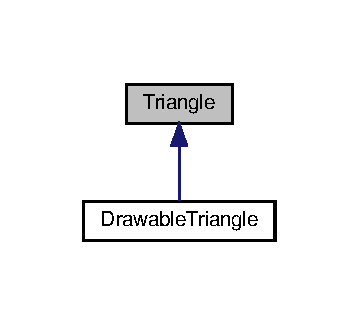
\includegraphics[width=172pt]{classTriangle__inherit__graph}
\end{center}
\end{figure}
\subsection*{Public Member Functions}
\begin{DoxyCompactItemize}
\item 
\hyperlink{classTriangle_a3bb081f3c4d90284e27e1005a2b33599}{Triangle} (const cg3\+::\+Point2\+Dd \&v1, const cg3\+::\+Point2\+Dd \&v2, const cg3\+::\+Point2\+Dd \&v3)
\begin{DoxyCompactList}\small\item\em Creates a node from 3 vertices. \end{DoxyCompactList}\item 
cg3\+::\+Point2\+Dd \hyperlink{classTriangle_a488beca5f5e516f4914f7ec118d2205e}{get\+V1} () const
\begin{DoxyCompactList}\small\item\em Returns the first vertex. \end{DoxyCompactList}\item 
cg3\+::\+Point2\+Dd \hyperlink{classTriangle_a6b22d833c2cc9b738793da637642bfd0}{get\+V2} () const
\begin{DoxyCompactList}\small\item\em Returns the second vertex. \end{DoxyCompactList}\item 
cg3\+::\+Point2\+Dd \hyperlink{classTriangle_ad63dee82c3268c96bb5a6d353675c133}{get\+V3} () const
\begin{DoxyCompactList}\small\item\em Returns the third vertex. \end{DoxyCompactList}\item 
cg3\+::\+Point2\+Dd \hyperlink{classTriangle_a4d120f7288b7051a1cf442268edd328d}{get\+Center} () const
\begin{DoxyCompactList}\small\item\em Returns the center of the triangle. \end{DoxyCompactList}\item 
cg3\+::\+Point2\+Dd \hyperlink{classTriangle_a0ac42109ff92fc5b907283e10d7946b2}{get\+Circumcenter} () const
\begin{DoxyCompactList}\small\item\em Returns the center of the triangle. \end{DoxyCompactList}\end{DoxyCompactItemize}
\subsection*{Protected Attributes}
\begin{DoxyCompactItemize}
\item 
\mbox{\Hypertarget{classTriangle_ac28fb730b25c0d52aac1d0faf12b1225}\label{classTriangle_ac28fb730b25c0d52aac1d0faf12b1225}} 
cg3\+::\+Point2\+Dd {\bfseries v1}
\item 
\mbox{\Hypertarget{classTriangle_a6d59f8e4f22f7436b6298051d24ae977}\label{classTriangle_a6d59f8e4f22f7436b6298051d24ae977}} 
cg3\+::\+Point2\+Dd {\bfseries v2}
\item 
\mbox{\Hypertarget{classTriangle_a8eb4459eb8ead2fc99742e2846d59264}\label{classTriangle_a8eb4459eb8ead2fc99742e2846d59264}} 
cg3\+::\+Point2\+Dd {\bfseries v3}
\end{DoxyCompactItemize}


\subsection{Detailed Description}
\hyperlink{classTriangle}{Triangle}. 

The triangle data structure is implemented by storing inserted points for the algorithm\+: it contains the 3 vertices in counter-\/clockwise order. This class implements getters and setters and two methods, one for the barycenter (used for the drawable) and one for the circumcenter (used for Voronoi). 

\subsection{Constructor \& Destructor Documentation}
\mbox{\Hypertarget{classTriangle_a3bb081f3c4d90284e27e1005a2b33599}\label{classTriangle_a3bb081f3c4d90284e27e1005a2b33599}} 
\index{Triangle@{Triangle}!Triangle@{Triangle}}
\index{Triangle@{Triangle}!Triangle@{Triangle}}
\subsubsection{\texorpdfstring{Triangle()}{Triangle()}}
{\footnotesize\ttfamily Triangle\+::\+Triangle (\begin{DoxyParamCaption}\item[{const cg3\+::\+Point2\+Dd \&}]{v1,  }\item[{const cg3\+::\+Point2\+Dd \&}]{v2,  }\item[{const cg3\+::\+Point2\+Dd \&}]{v3 }\end{DoxyParamCaption})}



Creates a node from 3 vertices. 


\begin{DoxyParams}[1]{Parameters}
\mbox{\tt in}  & {\em v1} & rightmost vertex \\
\hline
\mbox{\tt in}  & {\em v2} & topmost vertex \\
\hline
\mbox{\tt in}  & {\em v3} & leftmost vertex \\
\hline
\end{DoxyParams}


\subsection{Member Function Documentation}
\mbox{\Hypertarget{classTriangle_a4d120f7288b7051a1cf442268edd328d}\label{classTriangle_a4d120f7288b7051a1cf442268edd328d}} 
\index{Triangle@{Triangle}!get\+Center@{get\+Center}}
\index{get\+Center@{get\+Center}!Triangle@{Triangle}}
\subsubsection{\texorpdfstring{get\+Center()}{getCenter()}}
{\footnotesize\ttfamily cg3\+::\+Point2\+Dd Triangle\+::get\+Center (\begin{DoxyParamCaption}{ }\end{DoxyParamCaption}) const}



Returns the center of the triangle. 

\begin{DoxyReturn}{Returns}
center\+: the barycenter of the triangle 
\end{DoxyReturn}
\mbox{\Hypertarget{classTriangle_a0ac42109ff92fc5b907283e10d7946b2}\label{classTriangle_a0ac42109ff92fc5b907283e10d7946b2}} 
\index{Triangle@{Triangle}!get\+Circumcenter@{get\+Circumcenter}}
\index{get\+Circumcenter@{get\+Circumcenter}!Triangle@{Triangle}}
\subsubsection{\texorpdfstring{get\+Circumcenter()}{getCircumcenter()}}
{\footnotesize\ttfamily cg3\+::\+Point2\+Dd Triangle\+::get\+Circumcenter (\begin{DoxyParamCaption}{ }\end{DoxyParamCaption}) const}



Returns the center of the triangle. 

\begin{DoxyReturn}{Returns}
center\+: the circumcenter of the triangle 
\end{DoxyReturn}
\mbox{\Hypertarget{classTriangle_a488beca5f5e516f4914f7ec118d2205e}\label{classTriangle_a488beca5f5e516f4914f7ec118d2205e}} 
\index{Triangle@{Triangle}!get\+V1@{get\+V1}}
\index{get\+V1@{get\+V1}!Triangle@{Triangle}}
\subsubsection{\texorpdfstring{get\+V1()}{getV1()}}
{\footnotesize\ttfamily cg3\+::\+Point2\+Dd Triangle\+::get\+V1 (\begin{DoxyParamCaption}{ }\end{DoxyParamCaption}) const}



Returns the first vertex. 

\begin{DoxyReturn}{Returns}
v1\+: vertex 1 
\end{DoxyReturn}
\mbox{\Hypertarget{classTriangle_a6b22d833c2cc9b738793da637642bfd0}\label{classTriangle_a6b22d833c2cc9b738793da637642bfd0}} 
\index{Triangle@{Triangle}!get\+V2@{get\+V2}}
\index{get\+V2@{get\+V2}!Triangle@{Triangle}}
\subsubsection{\texorpdfstring{get\+V2()}{getV2()}}
{\footnotesize\ttfamily cg3\+::\+Point2\+Dd Triangle\+::get\+V2 (\begin{DoxyParamCaption}{ }\end{DoxyParamCaption}) const}



Returns the second vertex. 

\begin{DoxyReturn}{Returns}
v2\+: vertex 2 
\end{DoxyReturn}
\mbox{\Hypertarget{classTriangle_ad63dee82c3268c96bb5a6d353675c133}\label{classTriangle_ad63dee82c3268c96bb5a6d353675c133}} 
\index{Triangle@{Triangle}!get\+V3@{get\+V3}}
\index{get\+V3@{get\+V3}!Triangle@{Triangle}}
\subsubsection{\texorpdfstring{get\+V3()}{getV3()}}
{\footnotesize\ttfamily cg3\+::\+Point2\+Dd Triangle\+::get\+V3 (\begin{DoxyParamCaption}{ }\end{DoxyParamCaption}) const}



Returns the third vertex. 

\begin{DoxyReturn}{Returns}
v3\+: vertex 3 
\end{DoxyReturn}


The documentation for this class was generated from the following files\+:\begin{DoxyCompactItemize}
\item 
triangle.\+h\item 
triangle.\+cpp\end{DoxyCompactItemize}

\hypertarget{classTriangulation}{}\section{Triangulation Class Reference}
\label{classTriangulation}\index{Triangulation@{Triangulation}}
\subsection*{Public Member Functions}
\begin{DoxyCompactItemize}
\item 
\mbox{\Hypertarget{classTriangulation_a56118103ad86aa7b37d7a005892bfeca}\label{classTriangulation_a56118103ad86aa7b37d7a005892bfeca}} 
\hyperlink{classTriangulation_a56118103ad86aa7b37d7a005892bfeca}{Triangulation} ()
\begin{DoxyCompactList}\small\item\em Default constructor. \end{DoxyCompactList}\item 
\mbox{\Hypertarget{classTriangulation_ae1d2320b4ca69156f29a4e27dff921f1}\label{classTriangulation_ae1d2320b4ca69156f29a4e27dff921f1}} 
{\bfseries Triangulation} (const std\+::vector$<$ \hyperlink{classTriangle}{Triangle} $>$ \&triangles, const std\+::vector$<$ std\+::array$<$ int, max\+Adjacent\+Triangles $>$$>$ \&adjacencies)
\item 
void \hyperlink{classTriangulation_a2143e3330a01aeb0c49343e20a513e41}{add\+Triangle} (const \hyperlink{classTriangle}{Triangle} \&triangle)
\begin{DoxyCompactList}\small\item\em Add a triangle to the triangulation. \end{DoxyCompactList}\item 
std\+::vector$<$ \hyperlink{classTriangle}{Triangle} $>$ \& \hyperlink{classTriangulation_a9245c1ffae5777f76f51b217f267d594}{get\+Triangles} ()
\begin{DoxyCompactList}\small\item\em Returns the triangles of the triangulation. \end{DoxyCompactList}\item 
std\+::array$<$ int, max\+Adjacent\+Triangles $>$ \& \hyperlink{classTriangulation_a82cec4438c1f8b17f4d96160bdebb365}{get\+Adjacencies\+From\+Triangle} (const unsigned int triangle)
\begin{DoxyCompactList}\small\item\em Returns the adjacencies of the triangle. \end{DoxyCompactList}\item 
\mbox{\Hypertarget{classTriangulation_ad03152c349343f5f50542feeb05ead90}\label{classTriangulation_ad03152c349343f5f50542feeb05ead90}} 
void \hyperlink{classTriangulation_ad03152c349343f5f50542feeb05ead90}{clear\+Data\+Structure} ()
\begin{DoxyCompactList}\small\item\em Clears triangles and adjacencies but not the first triangle -\/ bounding triangle. \end{DoxyCompactList}\item 
void \hyperlink{classTriangulation_a77619bd20876c1b3322765ee5135e746}{add\+Adjacencies\+For\+New\+Triangle} (const int v1v2, const int v2v3, const int v3v1)
\begin{DoxyCompactList}\small\item\em Adds adjacencies for a new triangle. \end{DoxyCompactList}\item 
void \hyperlink{classTriangulation_a26221b1d8851ff0c1e0812a0d3c6afc1}{add\+Adjacencies\+For\+New\+Triangle} (const unsigned int triangle, const int v1v2, const int v2v3, const int v3v1, const unsigned int old)
\begin{DoxyCompactList}\small\item\em Adds adjacencies for a new triangle and replace old adjacencies when adding a triangle. \end{DoxyCompactList}\item 
void \hyperlink{classTriangulation_a489332eed4dd72b35b8763ce448d3f32}{add\+Adjacencies\+For\+New\+Triangle} (const unsigned int triangle, const int v1v2, const int v2v3, const int v3v1, const unsigned int old, const unsigned int old\+Adj)
\begin{DoxyCompactList}\small\item\em Adds adjacencies for a new triangle and replace old adjacencies when flipping edge. \end{DoxyCompactList}\item 
unsigned int \hyperlink{classTriangulation_a5cc5f70c9c66ce68e1a0140bab8dee68}{find\+Adjacency} (const unsigned int triangle, const unsigned int adjacent)
\begin{DoxyCompactList}\small\item\em Finds the edge where the triangle is adjacent to its adjacent triangle. \end{DoxyCompactList}\end{DoxyCompactItemize}
\subsection*{Protected Attributes}
\begin{DoxyCompactItemize}
\item 
\mbox{\Hypertarget{classTriangulation_a382d1156fe26a4460d4558a5f37c307c}\label{classTriangulation_a382d1156fe26a4460d4558a5f37c307c}} 
std\+::vector$<$ \hyperlink{classTriangle}{Triangle} $>$ {\bfseries triangles}
\item 
\mbox{\Hypertarget{classTriangulation_a81884b0393ebe68d4f58253d717c476b}\label{classTriangulation_a81884b0393ebe68d4f58253d717c476b}} 
std\+::vector$<$ std\+::array$<$ int, max\+Adjacent\+Triangles $>$ $>$ {\bfseries adjacencies}
\end{DoxyCompactItemize}


\subsection{Member Function Documentation}
\mbox{\Hypertarget{classTriangulation_a77619bd20876c1b3322765ee5135e746}\label{classTriangulation_a77619bd20876c1b3322765ee5135e746}} 
\index{Triangulation@{Triangulation}!add\+Adjacencies\+For\+New\+Triangle@{add\+Adjacencies\+For\+New\+Triangle}}
\index{add\+Adjacencies\+For\+New\+Triangle@{add\+Adjacencies\+For\+New\+Triangle}!Triangulation@{Triangulation}}
\subsubsection{\texorpdfstring{add\+Adjacencies\+For\+New\+Triangle()}{addAdjacenciesForNewTriangle()}\hspace{0.1cm}{\footnotesize\ttfamily [1/3]}}
{\footnotesize\ttfamily void Triangulation\+::add\+Adjacencies\+For\+New\+Triangle (\begin{DoxyParamCaption}\item[{const int}]{v1v2,  }\item[{const int}]{v2v3,  }\item[{const int}]{v3v1 }\end{DoxyParamCaption})}



Adds adjacencies for a new triangle. 


\begin{DoxyParams}[1]{Parameters}
\mbox{\tt in}  & {\em v1v2} & the adjacent triangle index in edge v1v2 \\
\hline
\mbox{\tt in}  & {\em v2v3} & the adjacent triangle index in edge v2v3 \\
\hline
\mbox{\tt in}  & {\em v3v1} & the adjacent triangle index in edge v3v1 \\
\hline
\end{DoxyParams}
\mbox{\Hypertarget{classTriangulation_a26221b1d8851ff0c1e0812a0d3c6afc1}\label{classTriangulation_a26221b1d8851ff0c1e0812a0d3c6afc1}} 
\index{Triangulation@{Triangulation}!add\+Adjacencies\+For\+New\+Triangle@{add\+Adjacencies\+For\+New\+Triangle}}
\index{add\+Adjacencies\+For\+New\+Triangle@{add\+Adjacencies\+For\+New\+Triangle}!Triangulation@{Triangulation}}
\subsubsection{\texorpdfstring{add\+Adjacencies\+For\+New\+Triangle()}{addAdjacenciesForNewTriangle()}\hspace{0.1cm}{\footnotesize\ttfamily [2/3]}}
{\footnotesize\ttfamily void Triangulation\+::add\+Adjacencies\+For\+New\+Triangle (\begin{DoxyParamCaption}\item[{const unsigned int}]{triangle,  }\item[{const int}]{v1v2,  }\item[{const int}]{v2v3,  }\item[{const int}]{v3v1,  }\item[{const unsigned int}]{old }\end{DoxyParamCaption})}



Adds adjacencies for a new triangle and replace old adjacencies when adding a triangle. 


\begin{DoxyParams}[1]{Parameters}
\mbox{\tt in}  & {\em v1v2} & the adjacent triangle index in edge v1v2 \\
\hline
\mbox{\tt in}  & {\em v2v3} & the adjacent triangle index in edge v2v3 \\
\hline
\mbox{\tt in}  & {\em v3v1} & the adjacent triangle index in edge v3v1 \\
\hline
\mbox{\tt in}  & {\em old} & the old triangle index that must be replaced in the adjacencies \\
\hline
\end{DoxyParams}
\mbox{\Hypertarget{classTriangulation_a489332eed4dd72b35b8763ce448d3f32}\label{classTriangulation_a489332eed4dd72b35b8763ce448d3f32}} 
\index{Triangulation@{Triangulation}!add\+Adjacencies\+For\+New\+Triangle@{add\+Adjacencies\+For\+New\+Triangle}}
\index{add\+Adjacencies\+For\+New\+Triangle@{add\+Adjacencies\+For\+New\+Triangle}!Triangulation@{Triangulation}}
\subsubsection{\texorpdfstring{add\+Adjacencies\+For\+New\+Triangle()}{addAdjacenciesForNewTriangle()}\hspace{0.1cm}{\footnotesize\ttfamily [3/3]}}
{\footnotesize\ttfamily void Triangulation\+::add\+Adjacencies\+For\+New\+Triangle (\begin{DoxyParamCaption}\item[{const unsigned int}]{triangle,  }\item[{const int}]{v1v2,  }\item[{const int}]{v2v3,  }\item[{const int}]{v3v1,  }\item[{const unsigned int}]{old,  }\item[{const unsigned int}]{old\+Adj }\end{DoxyParamCaption})}



Adds adjacencies for a new triangle and replace old adjacencies when flipping edge. 


\begin{DoxyParams}[1]{Parameters}
\mbox{\tt in}  & {\em v1v2} & the adjacent triangle index in edge v1v2 \\
\hline
\mbox{\tt in}  & {\em v2v3} & the adjacent triangle index in edge v2v3 \\
\hline
\mbox{\tt in}  & {\em v3v1} & the adjacent triangle index in edge v3v1 \\
\hline
\mbox{\tt in}  & {\em old} & the old triangle index that must be replaced in the adjacencies \\
\hline
\mbox{\tt in}  & {\em old\+Adj} & the old adjacent triangle index that must be replaced in the adjacencies \\
\hline
\end{DoxyParams}
\mbox{\Hypertarget{classTriangulation_a2143e3330a01aeb0c49343e20a513e41}\label{classTriangulation_a2143e3330a01aeb0c49343e20a513e41}} 
\index{Triangulation@{Triangulation}!add\+Triangle@{add\+Triangle}}
\index{add\+Triangle@{add\+Triangle}!Triangulation@{Triangulation}}
\subsubsection{\texorpdfstring{add\+Triangle()}{addTriangle()}}
{\footnotesize\ttfamily void Triangulation\+::add\+Triangle (\begin{DoxyParamCaption}\item[{const \hyperlink{classTriangle}{Triangle} \&}]{triangle }\end{DoxyParamCaption})}



Add a triangle to the triangulation. 


\begin{DoxyParams}[1]{Parameters}
\mbox{\tt in}  & {\em triangle} & triangle to add \\
\hline
\end{DoxyParams}
\mbox{\Hypertarget{classTriangulation_a5cc5f70c9c66ce68e1a0140bab8dee68}\label{classTriangulation_a5cc5f70c9c66ce68e1a0140bab8dee68}} 
\index{Triangulation@{Triangulation}!find\+Adjacency@{find\+Adjacency}}
\index{find\+Adjacency@{find\+Adjacency}!Triangulation@{Triangulation}}
\subsubsection{\texorpdfstring{find\+Adjacency()}{findAdjacency()}}
{\footnotesize\ttfamily unsigned int Triangulation\+::find\+Adjacency (\begin{DoxyParamCaption}\item[{const unsigned int}]{triangle,  }\item[{const unsigned int}]{adjacent }\end{DoxyParamCaption})}



Finds the edge where the triangle is adjacent to its adjacent triangle. 


\begin{DoxyParams}[1]{Parameters}
\mbox{\tt in}  & {\em triangle} & the index to be tested \\
\hline
\mbox{\tt in}  & {\em adjacent} & the adjacent triangle where the adjacency must be checked \\
\hline
\end{DoxyParams}
\begin{DoxyReturn}{Returns}
adjacency\+: the edge where the triangle is adjacent to the adjacent triangle 
\end{DoxyReturn}
\mbox{\Hypertarget{classTriangulation_a82cec4438c1f8b17f4d96160bdebb365}\label{classTriangulation_a82cec4438c1f8b17f4d96160bdebb365}} 
\index{Triangulation@{Triangulation}!get\+Adjacencies\+From\+Triangle@{get\+Adjacencies\+From\+Triangle}}
\index{get\+Adjacencies\+From\+Triangle@{get\+Adjacencies\+From\+Triangle}!Triangulation@{Triangulation}}
\subsubsection{\texorpdfstring{get\+Adjacencies\+From\+Triangle()}{getAdjacenciesFromTriangle()}}
{\footnotesize\ttfamily std\+::array$<$ int, max\+Adjacent\+Triangles $>$ \& Triangulation\+::get\+Adjacencies\+From\+Triangle (\begin{DoxyParamCaption}\item[{const unsigned int}]{triangle }\end{DoxyParamCaption})}



Returns the adjacencies of the triangle. 


\begin{DoxyParams}[1]{Parameters}
\mbox{\tt in}  & {\em triangle} & the index of the triangle \\
\hline
\end{DoxyParams}
\begin{DoxyReturn}{Returns}
adjacencies\+: the array containing the adjacencies for the triangle 
\end{DoxyReturn}
\mbox{\Hypertarget{classTriangulation_a9245c1ffae5777f76f51b217f267d594}\label{classTriangulation_a9245c1ffae5777f76f51b217f267d594}} 
\index{Triangulation@{Triangulation}!get\+Triangles@{get\+Triangles}}
\index{get\+Triangles@{get\+Triangles}!Triangulation@{Triangulation}}
\subsubsection{\texorpdfstring{get\+Triangles()}{getTriangles()}}
{\footnotesize\ttfamily std\+::vector$<$ \hyperlink{classTriangle}{Triangle} $>$ \& Triangulation\+::get\+Triangles (\begin{DoxyParamCaption}{ }\end{DoxyParamCaption})}



Returns the triangles of the triangulation. 

\begin{DoxyReturn}{Returns}
triangles\+: the array of triangles 
\end{DoxyReturn}


The documentation for this class was generated from the following files\+:\begin{DoxyCompactItemize}
\item 
triangulation.\+h\item 
triangulation.\+cpp\end{DoxyCompactItemize}

%--- End generated contents ---

% Index
\backmatter
\newpage
\phantomsection
\clearemptydoublepage
\addcontentsline{toc}{chapter}{Index}
\printindex

\end{document}
